% vim: set spell spelllang=en tw=100 et sw=4 sts=4 foldmethod=marker foldmarker={{{,}}} :

\documentclass{beamer}

\usepackage{tikz}
\usepackage{xcolor}
\usepackage{complexity}
\usepackage{hyperref}
\usepackage{microtype}
\usepackage{amsmath}                   % \operatorname
\usepackage{amsfonts}                  % \mathcal
\usepackage{amssymb}                   % \nexists
\usepackage[vlined]{algorithm2e} % algorithms
\usepackage{centernot}
\usepackage{listings}
\usepackage{csquotes}

\RequirePackage[tt=false, type1=true]{libertine}
\RequirePackage[varqu]{zi4}
\RequirePackage[libertine]{newtxmath}
\RequirePackage[T1]{fontenc}

\usetikzlibrary{shapes, arrows, shadows, calc, positioning, fit}
\usetikzlibrary{decorations.pathreplacing, decorations.pathmorphing, shapes.misc}
\usetikzlibrary{tikzmark}

\definecolor{uofguniversityblue}{rgb}{0, 0.219608, 0.396078}

\definecolor{uofgheather}{rgb}{0.356863, 0.32549, 0.490196}
\definecolor{uofgaquamarine}{rgb}{0.603922, 0.72549, 0.678431}
\definecolor{uofgslate}{rgb}{0.309804, 0.34902, 0.380392}
\definecolor{uofgrose}{rgb}{0.823529, 0.470588, 0.709804}
\definecolor{uofgmocha}{rgb}{0.709804, 0.564706, 0.47451}
\definecolor{uofgsandstone}{rgb}{0.321569, 0.278431, 0.231373}
\definecolor{uofgforest}{rgb}{0, 0.2, 0.129412}
\definecolor{uofglawn}{rgb}{0.517647, 0.741176, 0}
\definecolor{uofgcobalt}{rgb}{0, 0.615686, 0.92549}
\definecolor{uofgturquoise}{rgb}{0, 0.709804, 0.819608}
\definecolor{uofgsunshine}{rgb}{1.0, 0.862745, 0.211765}
\definecolor{uofgpumpkin}{rgb}{1.0, 0.72549, 0.282353}
\definecolor{uofgthistle}{rgb}{0.584314, 0.070588, 0.447059}
\definecolor{uofgrust}{rgb}{0.603922, 0.227451, 0.023529}
\definecolor{uofgburgundy}{rgb}{0.490196, 0.133333, 0.223529}
\definecolor{uofgpillarbox}{rgb}{0.701961, 0.047059, 0}
\definecolor{uofglavendar}{rgb}{0.356863, 0.301961, 0.580392}

\tikzset{vertex/.style={draw, circle, inner sep=0pt, minimum size=0.5cm, font=\small\bfseries}}
\tikzset{notvertex/.style={vertex, color=white, text=black}}
\tikzset{plainvertex/.style={vertex}}
\tikzset{vertexc1/.style={vertex, fill=uofgburgundy, text=white}}
\tikzset{vertexc2/.style={vertex, fill=uofgsandstone, text=white}}
\tikzset{vertexc3/.style={vertex, fill=uofgforest, text=white}}
\tikzset{vertexc4/.style={vertex, fill=uofgheather, text=white}}
\tikzset{edge/.style={color=black!50!white}}
\tikzset{bedge/.style={ultra thick}}

% {{{ theme things
\useoutertheme[footline=authortitle]{miniframes}
\useinnertheme{rectangles}

\setbeamerfont{block title}{size={}}
\setbeamerfont{title}{size=\large,series=\bfseries}
\setbeamerfont{section title}{size=\large,series=\mdseries}
\setbeamerfont{author}{size=\normalsize,series=\mdseries}
\setbeamercolor*{structure}{fg=uofguniversityblue}
\setbeamercolor*{palette primary}{use=structure,fg=black,bg=white}
\setbeamercolor*{palette secondary}{use=structure,fg=white,bg=uofgcobalt}
\setbeamercolor*{palette tertiary}{use=structure,fg=white,bg=uofguniversityblue}
\setbeamercolor*{palette quaternary}{fg=white,bg=black}

\setbeamercolor*{titlelike}{parent=palette primary}

\beamertemplatenavigationsymbolsempty

\setbeamertemplate{title page}
{
    \begin{tikzpicture}[remember picture, overlay]
        \node at (current page.north west) {
            \begin{tikzpicture}[remember picture, overlay]
                \fill [fill=uofguniversityblue, anchor=north west] (0, 0) rectangle (\paperwidth, -2.6cm);
            \end{tikzpicture}
        };

        \node (logo) [anchor=north east, shift={(-0.6cm,-0.4cm)}] at (current page.north east) {
            \begin{minipage}{0.20\paperwidth}
                \begin{center}
                
\includegraphics[keepaspectratio=true,scale=0.35]{UoG_keyline.pdf} \\[0.15cm]
                
\includegraphics[keepaspectratio=true,scale=0.8]{UStA_Logo_SP.eps}
                \end{center}
            \end{minipage}
        };

        \node [anchor=west, xshift=0.2cm, yshift=0.2cm] at (current page.west |- logo.west) {
            \begin{minipage}{0.65\paperwidth}\raggedright
                {\usebeamerfont{title}\usebeamercolor[white]{}\inserttitle}\\[0.1cm]
                {\usebeamerfont{author}\usebeamercolor[white]{}\insertauthor}
            \end{minipage}
        };
    \end{tikzpicture}
}

\setbeamertemplate{section page}
{
    \begin{centering}
        \begin{beamercolorbox}[sep=12pt,center]{part title}
            \usebeamerfont{section title}\insertsection\par
        \end{beamercolorbox}
    \end{centering}
}

\newcommand{\frameofframes}{/}
\newcommand{\setframeofframes}[1]{\renewcommand{\frameofframes}{#1}}

\makeatletter
\setbeamertemplate{footline}
{%
    \begin{beamercolorbox}[colsep=1.5pt]{upper separation line foot}
    \end{beamercolorbox}
    \begin{beamercolorbox}[ht=2.5ex,dp=1.125ex,%
        leftskip=.3cm,rightskip=.3cm plus1fil]{author in head/foot}%
        \leavevmode{\usebeamerfont{author in head/foot}\insertshortauthor}%
        \hfill%
        {\usebeamerfont{institute in head/foot}\usebeamercolor[fg]{institute in head/foot}\insertshortinstitute}%
    \end{beamercolorbox}%
    \begin{beamercolorbox}[ht=2.5ex,dp=1.125ex,%
        leftskip=.3cm,rightskip=.3cm plus1fil]{title in head/foot}%
        {\usebeamerfont{title in head/foot}\insertshorttitle}%
        \hfill%
        {\usebeamerfont{frame number}\usebeamercolor[fg]{frame number}\insertframenumber~\frameofframes~\inserttotalframenumber}
    \end{beamercolorbox}%
    \begin{beamercolorbox}[colsep=1.5pt]{lower separation line foot}
    \end{beamercolorbox}
}

\makeatletter
\newenvironment{nearlyplainframe}[2][]{
    \def\beamer@entrycode{\vspace*{-\headheight}\vspace*{3pt}}
    \setbeamertemplate{headline}
    {%
        \begin{beamercolorbox}[colsep=1.5pt]{upper separation line head}
        \end{beamercolorbox}
        \begin{beamercolorbox}[ht=0.5ex,dp=0.125ex,%
            leftskip=.3cm,rightskip=.3cm plus1fil]{title in head/foot}%
        \end{beamercolorbox}%
        \begin{beamercolorbox}[ht=0.5ex,dp=0.125ex,%
            leftskip=.3cm,rightskip=.3cm plus1fil]{author in head/foot}%
        \end{beamercolorbox}%
        \begin{beamercolorbox}[colsep=1.5pt]{lower separation line head}
        \end{beamercolorbox}
        \vspace*{\headheight}
    }

    \setbeamertemplate{footline}
    {%
        \begin{beamercolorbox}[colsep=1.5pt]{upper separation line foot}
        \end{beamercolorbox}
        \begin{beamercolorbox}[ht=0.5ex,dp=0.125ex,%
            leftskip=.3cm,rightskip=.3cm plus1fil]{author in head/foot}%
        \end{beamercolorbox}%
        \begin{beamercolorbox}[ht=0.5ex,dp=0.125ex,%
            leftskip=.3cm,rightskip=.3cm plus1fil]{title in head/foot}%
        \end{beamercolorbox}%
        \begin{beamercolorbox}[colsep=1.5pt]{lower separation line foot}
        \end{beamercolorbox}
    }

    \begin{frame}[#1]{#2}
    }{
    \end{frame}
}
\makeatother

\makeatletter
\newenvironment{justborderframe}[2][]{
    \def\beamer@entrycode{\vspace*{-\headheight}}
    \setbeamertemplate{headline}
    {%
        \begin{beamercolorbox}[colsep=1.5pt]{upper separation line head}
        \end{beamercolorbox}
        \begin{beamercolorbox}[ht=0.5ex,dp=0.125ex,%
            leftskip=.3cm,rightskip=.3cm plus1fil]{title in head/foot}%
        \end{beamercolorbox}%
        \begin{beamercolorbox}[ht=0.5ex,dp=0.125ex,%
            leftskip=.3cm,rightskip=.3cm plus1fil]{author in head/foot}%
        \end{beamercolorbox}%
        \begin{beamercolorbox}[colsep=1.5pt]{lower separation line head}
        \end{beamercolorbox}
        \vspace*{\headheight}
    }

    \setbeamertemplate{footline}
    {%
        \begin{beamercolorbox}[colsep=1.5pt]{upper separation line foot}
        \end{beamercolorbox}
        \begin{beamercolorbox}[ht=0.5ex,dp=0.125ex,%
            leftskip=.3cm,rightskip=.3cm plus1fil]{author in head/foot}%
        \end{beamercolorbox}%
        \begin{beamercolorbox}[ht=0.5ex,dp=0.125ex,%
            leftskip=.3cm,rightskip=.3cm plus1fil]{title in head/foot}%
        \end{beamercolorbox}%
        \begin{beamercolorbox}[colsep=1.5pt]{lower separation line foot}
        \end{beamercolorbox}
    }

    \begin{frame}[#1]{}
    }{
    \end{frame}
}
\makeatother


% }}}

\author{Blair Archibald \and Fraser Dunlop \and Ruth Hoffmann \and Ciaran McCreesh \and Patrick
Prosser \and James Trimble}
\title{Sequential and Parallel Solution-Biased Search for Subgraph Algorithms}

\begin{document}

{
    \usebackgroundtemplate{
        \tikz[overlay, remember picture]
        \node[at=(current page.south), anchor=south, inner sep=0pt]{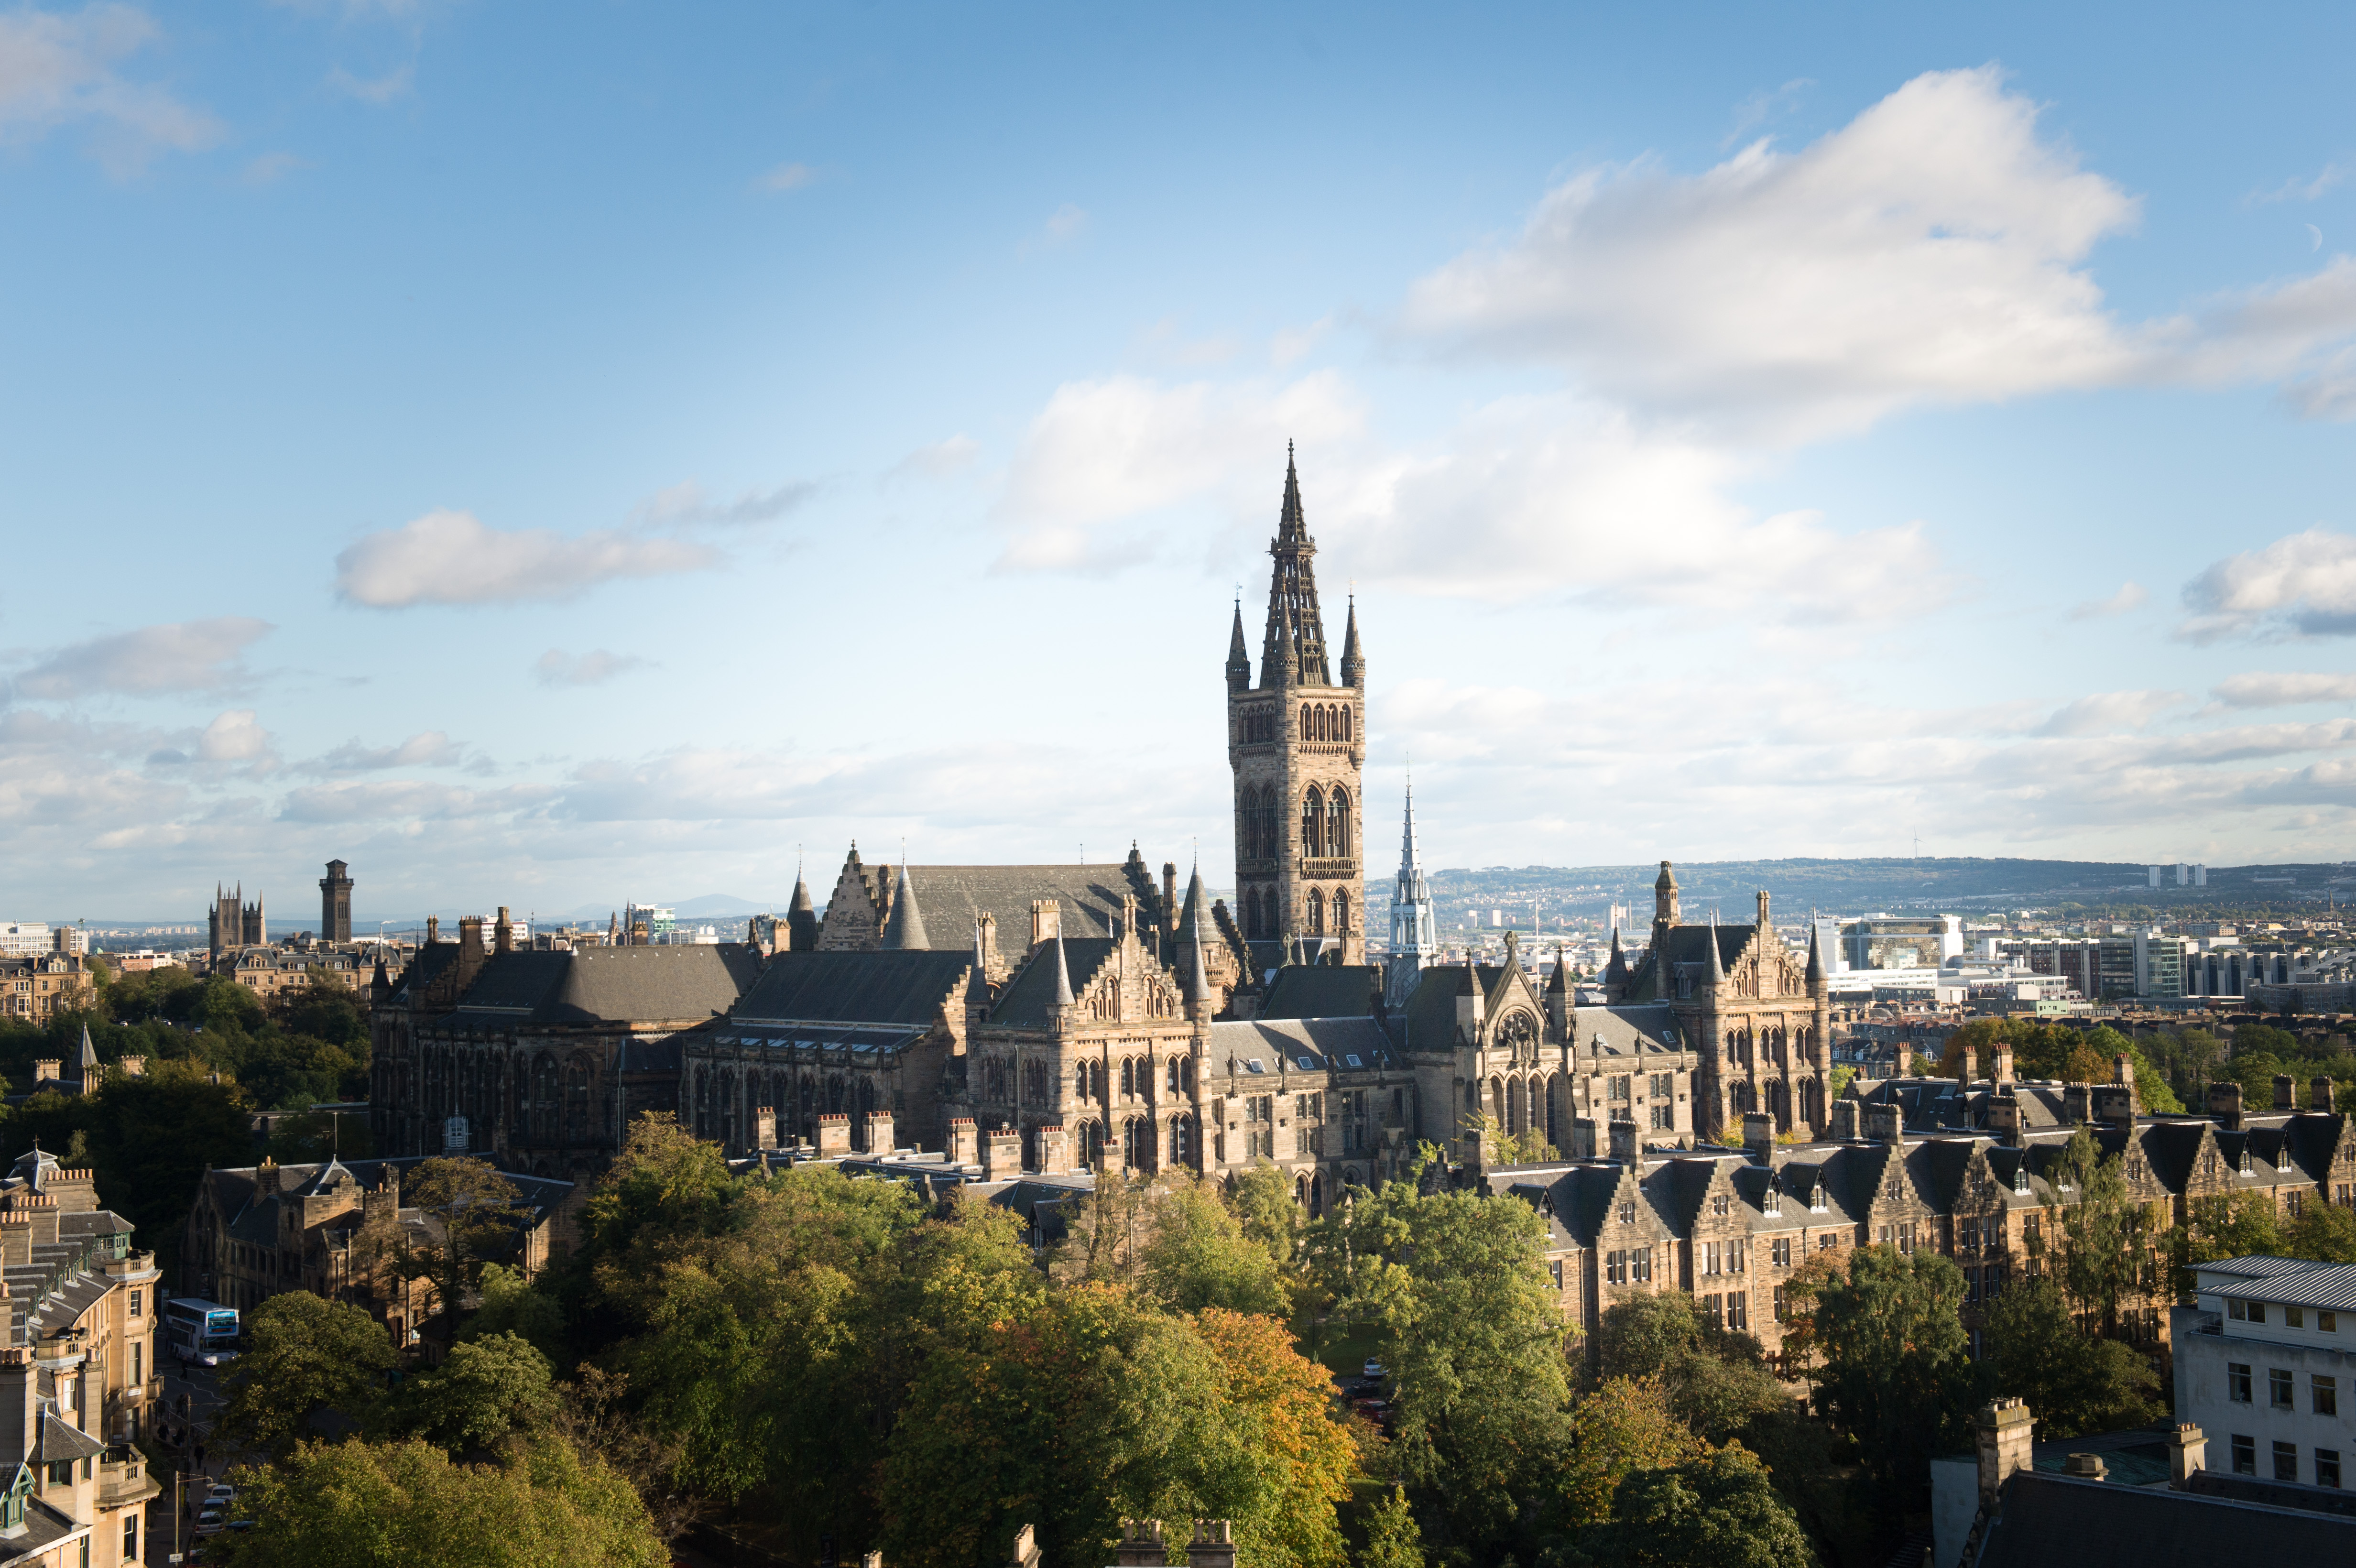
\includegraphics[keepaspectratio=true, height=\paperheight]{background.jpg}};
    }
    \begin{frame}[plain,noframenumbering]
        \titlepage
    \end{frame}
}

\begin{frame}{Subgraph Isomorphism}
    \centering
    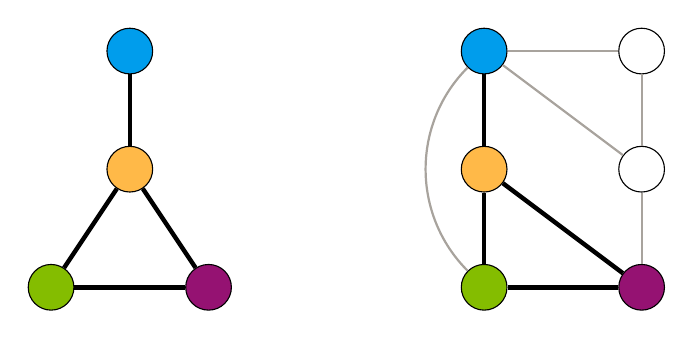
\begin{tikzpicture}
        \node [draw, circle, fill=uofgcobalt, inner sep=4pt, font=\bfseries] (Na) at (1,  0) {\vphantom{1}};
        \node [draw, circle, fill=uofgpumpkin, inner sep=4pt, font=\bfseries] (Nb) at (1, -1.5) {\vphantom{1}};
        \node [draw, circle, fill=uofglawn, inner sep=4pt, font=\bfseries] (Nc) at (0, -3) {\vphantom{1}};
        \node [draw, circle, fill=uofgthistle, inner sep=4pt, font=\bfseries] (Nd) at (2, -3) {\vphantom{1}};

        \draw [ultra thick] (Na) -- (Nb);
        \draw [ultra thick] (Nb) -- (Nc);
        \draw [ultra thick] (Nc) -- (Nd);
        \draw [ultra thick] (Nb) -- (Nd);

        \node [draw, circle, fill=uofgcobalt, inner sep=4pt, font=\bfseries] (N1) at (5.5,  0) {\vphantom{1}};
        \node [draw, circle, fill=white, inner sep=4pt, font=\bfseries] (N2) at (7.5,  0) {\vphantom{1}};
        \node [draw, circle, fill=uofgpumpkin, inner sep=4pt, font=\bfseries] (N3) at (5.5, -1.5) {\vphantom{1}};
        \node [draw, circle, fill=white, inner sep=4pt, font=\bfseries] (N4) at (7.5, -1.5) {\vphantom{1}};
        \node [draw, circle, fill=uofglawn, inner sep=4pt, font=\bfseries] (N5) at (5.5, -3) {\vphantom{1}};
        \node [draw, circle, fill=uofgthistle, inner sep=4pt, font=\bfseries] (N6) at (7.5, -3) {\vphantom{1}};

        \draw [thick, color=uofgsandstone!50] (N1) -- (N2);
        \draw [ultra thick] (N1) -- (N3);
        \draw [thick, color=uofgsandstone!50] (N1) -- (N4);
        \draw [thick, color=uofgsandstone!50] (N2) -- (N4);
        \draw [ultra thick] (N3) -- (N5);
        \draw [ultra thick] (N3) -- (N6);
        \draw [thick, color=uofgsandstone!50] (N4) -- (N6);
        \draw [ultra thick] (N5) -- (N6);
        \draw [thick, color=uofgsandstone!50] (N1) to [in=135, out=225] (N5);
    \end{tikzpicture}
\end{frame}

\begin{frame}{Subgraph Finding, as a Constraint Program}
    \begin{itemize}
        \item A variable for each pattern vertex. The domains are all of the target vertices.
        \item At least two sets of constraints:
            \begin{itemize}
                \item Adjacent pairs of vertices must be mapped to adjacent pairs of vertices.
                \item All different.
            \end{itemize}
        \item Then we get clever:
            \begin{itemize}
                \item Extra constraints about degrees, paths, \ldots
                \item Very good variable- and value-ordering heuristics
            \end{itemize}
    \end{itemize}
\end{frame}

\begin{frame}{The Glasgow Subgraph Solver}
    \begin{center}
        \url{https://github.com/ciaranm/glasgow-subgraph-solver}
    \end{center}

    \begin{itemize}
        \item Subgraph isomorphism, and all its variants (induced / non-induced, homomorphism,
            locally injective, labels, side constraints, directed, \ldots).
        \item Also special algorithms for clique.
    \end{itemize}
\end{frame}

\begin{frame}{Value-Ordering Heuristics}
    \begin{itemize}
        \item Largest target degree first.
    \end{itemize}
\end{frame}

\begin{frame}{Sanity Check}
    \begin{center}
        \includegraphics<1>{gen-graph-value-ordering.pdf}%
        \includegraphics<2>{gen-graph-value-ordering-unsat.pdf}
    \end{center}
\end{frame}

\begin{frame}{However\ldots}
    \begin{itemize}
        \item What if several vertices have the same degree?
        \item Is a vertex of degree $10$ really that much better than a vertex of degree $9$?
    \end{itemize}
\end{frame}

\begin{frame}{Discrepancy Search?}
    \begin{center}
        \includegraphics<1>{gen-graph-value-ordering-dds.pdf}%
        \includegraphics<2>{gen-graph-value-ordering-dds-unsat.pdf}%
        \includegraphics<3>{gen-graph-value-ordering-dds-scatter.pdf}
    \end{center}
\end{frame}

\begin{frame}{Value-Ordering Heuristics as Distributions}
    \begin{itemize}
        \item Traditional view: value-ordering defines a search order.
        \item New view: value-ordering defines \textcolor{uofgcobalt}{what proportion of the search
            effort} should be spent on different subproblems.
    \end{itemize}
\end{frame}

\begin{frame}{A Slightly Random Value-Ordering Heuristic}
    \only<1>{
    \[ p(v') = \frac{2^{\deg(v')}}{\sum_{w \in D_v}{2^{\deg(w)}}} \]
    \begin{itemize}
        \item Equally likely to pick between two vertices of degree $d$.
        \item Twice as likely to select a vertex of degree $d$ than a vertex of degree $d - 1$.
        \item In the paper: \textcolor{uofgcobalt}{solution density} and expected distribution of solutions.
    \end{itemize}}\only<2>{
    \begin{center}
        \includegraphics<2>{gen-graph-bias-scatter.pdf}%
    \end{center}}
\end{frame}

\begin{frame}{Restarts and Nogood Recording}
    \begin{itemize}
        \item Aggressive restarts: every 100ms.
        \item Nogood recording and 2WL to avoid repeating work.
    \end{itemize}
\end{frame}

\begin{frame}{Is It Better?}
    \begin{center}
        \includegraphics<1>{gen-graph-sbs.pdf}%
        \includegraphics<2>{gen-graph-sbs-unsat.pdf}%
        \includegraphics<3>{gen-graph-sbs-scatter.pdf}%
    \end{center}
\end{frame}

\begin{frame}{Parallel Search}
    \begin{itemize}
        \item Each thread gets its own random seed.
        \item Barrier synchronise on restarts.
        \item Share nogoods.
    \end{itemize}
\end{frame}

\begin{frame}{Is It Even Betterer?}
    \includegraphics<1>{gen-graph-par-scatter.pdf}%
    \includegraphics<2>{gen-graph-par.pdf}%
    \includegraphics<3>{gen-graph-dist.pdf}%
\end{frame}

\begin{frame}{Broader Perspective}
    \begin{itemize}
        \item Also good for maximum common subgraph algorithms.
        \item Does this work for CP in general?
        \item Can we finally kill off vanilla sequential backtracking search?
    \end{itemize}
\end{frame}

{
    \usebackgroundtemplate{
        \tikz[overlay, remember picture]
        \node[at=(current page.south), anchor=south, inner
        sep=0pt]{\includegraphics[keepaspectratio=true, width=\paperwidth]{background2.jpg}};
    }

    \begin{frame}[plain,noframenumbering]
        \begin{tikzpicture}[remember picture, overlay]
            \node at (current page.north west) {
                \begin{tikzpicture}[remember picture, overlay]
                    \fill [fill=uofguniversityblue, anchor=north west] (0, 0) rectangle (\paperwidth, -2.6cm);
                \end{tikzpicture}
            };

            \node (logo) [anchor=north east, shift={(-0.6cm,-0.6cm)}] at (current page.north east) {
                
\includegraphics[keepaspectratio=true,scale=0.7]{UoG_keyline.pdf}
            };

            \node [anchor=north west, shift={(0.6cm,-0.8cm)}] at (current page.north west) {
                \textcolor{white}{\url{http://www.dcs.gla.ac.uk/~ciaran}}
            };

            \node [anchor=north west, shift={(0.6cm,-1.4cm)}] at (current page.north west) {
                    \textcolor{white}{\href{mailto:ciaran.mccreesh@glasgow.ac.uk}{\nolinkurl{ciaran.mccreesh@glasgow.ac.uk}}}
            };
        \end{tikzpicture}
    \end{frame}
}

\end{document}

